Having validated the PINN approach by solving the homogeneous system, we now turn our attention toward a more advanced
inverse problem for which neural networks are particularly well-suited. In this scheme, we are given initial conditions 
along with height and velocity measurements over some unknown bathymetry which we wish to reconstruct via a PINN. 

Our test case is the inhomogeneous SWE system with a non-trivial sinusoidal bathymetry function

$$
B(x) = -\frac{1}{4} + \frac{1}{4} \cos{\left( \frac{\pi x}{5} \right)}.
$$

\noindent along with initial conditions

$$
h(x, 0) = \frac{1}{2} + \frac{2}{5} \sin{\left( \frac{\pi x}{10} \right)} \quad \text{and} \quad v(x, 0) = 0.
$$

As before, we use a neural network for the wave height and velocity with three hidden layers with 20 neurons each, along
with a second identical network (with only a single output neuron) to represent the inferred bathymetry. After training 
the network with 1000 height and velocity measurements over 100000 Adam iterations and 18000 L-BFGS iterations with a 
learning rate of $0.001$ , we obtain a mean residual value

$$
\lVert R(\Omega) \rVert_2 = 0.004952.
$$

\noindent again over a randomly sampled subset $\Omega$ of the computational domain. 
\textbf{TODO: Mention 0.05647 L2 relative error.}

% \begin{figure}[h]
%     \centering
%     \begin{subfigure}[b]{0.45\textwidth}
%         \centering
%         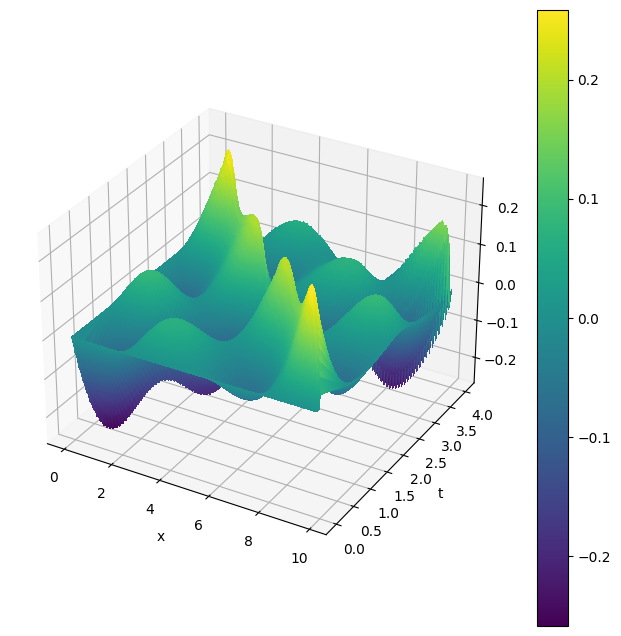
\includegraphics[width=\textwidth]{images/inhomogeneous_swe_pseudospectral_velocity.png}
%         \caption{Reference wave velocity}
%         \label{fig:inhomogeneous_pseudospectral_swe_velocity}
%     \end{subfigure}
%     \hfill
%     \begin{subfigure}[b]{0.45\textwidth}
%         \centering
%         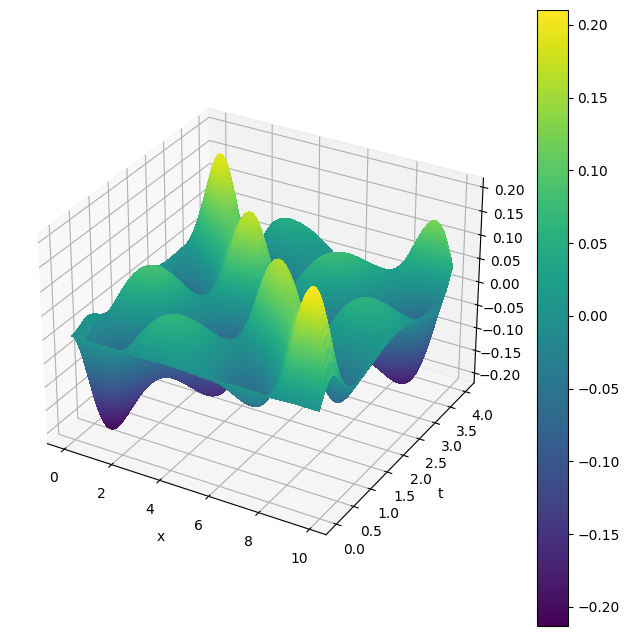
\includegraphics[width=\textwidth]{images/inhomogeneous_swe_pinn_velocity.png}
%         \caption{PINN wave velocity}
%         \label{fig:inhomogeneous_pinn_swe_velocity}
%     \end{subfigure}
%     \begin{subfigure}[b]{0.45\textwidth}
%         \centering
%         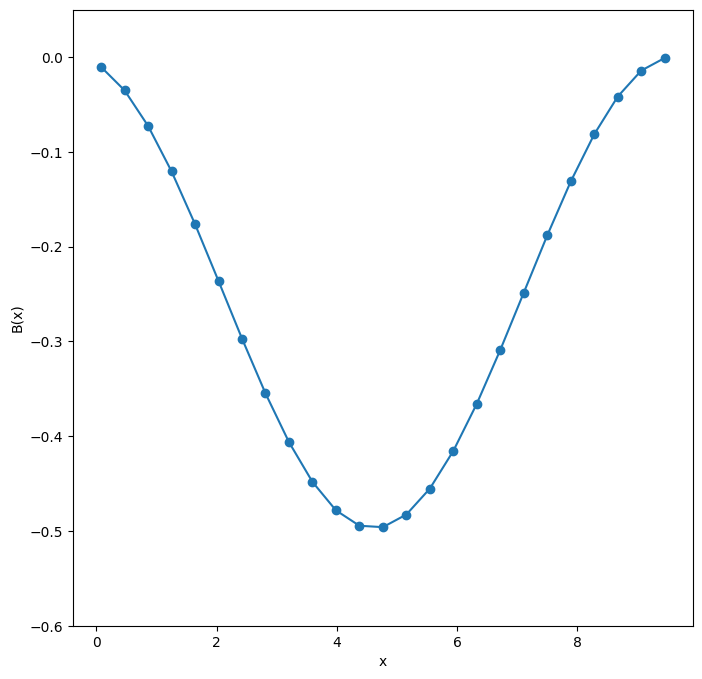
\includegraphics[width=\textwidth]{images/inhomogeneous_swe_pseudospectral_bathymetry.png}
%         \caption{Reference wave bathymetry}
%         \label{fig:inhomogeneous_pseudospectral_swe_bathymetry}
%     \end{subfigure}
%     \hfill
%     \begin{subfigure}[b]{0.45\textwidth}
%         \centering
%         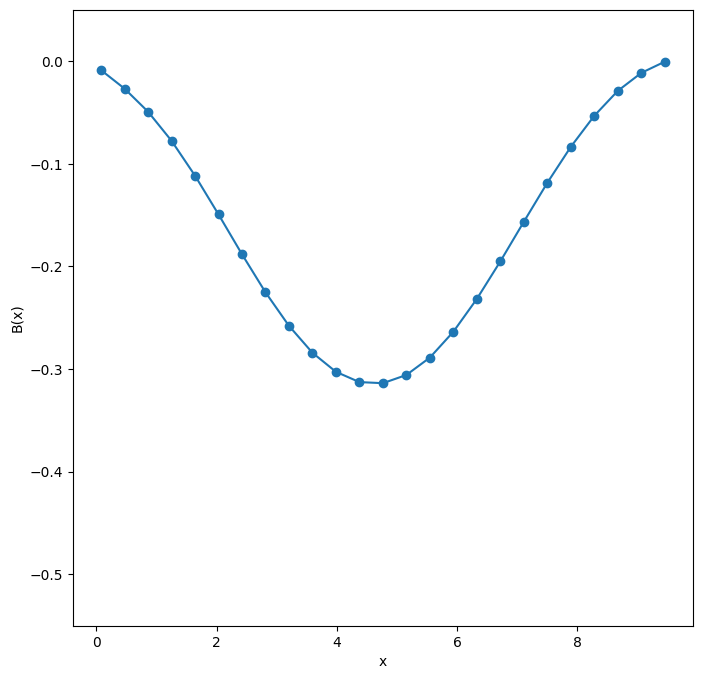
\includegraphics[width=\textwidth]{images/inhomogeneous_swe_pinn_bathymetry.png}
%         \caption{Inferred PINN bathymetry}
%         \label{fig:inhomogeneous_pinn_swe_bathymetry}
%     \end{subfigure}
%     \caption{Pseudospectral and PINN solutions for the inhomogeneous SWE system.}
%     \label{fig:inhomogeneous_swe_solution}
% \end{figure}